\section{Neural Networks and PDFs}
\label{sec:Init}


In the following, we prepare the ground for the study of the training dynamics
of neural networks used in the NNPDF framework. We start by presenting briefly
the inverse problem of PDF determination using data depending linearly on the PDFs,
setting the notation and introducing the statistical
vocabulary used in the rest of this study. We then discuss some
statistical aspects of the neural networks at initialisation, which will help us
understand the implications in the training process. These properties, derived
in the large-width limit~\cite{lee2019wide,jacot2018neural}, are analysed for the
specific architecture used in the NNPDF methodology. An exhaustive and detailed
review of wide-network properties is beyond the scope of this work, and the
reader is encouraged to refer to Ref.~\cite{Roberts:2021fes} for a comprehensive
review.

\subsection{The 1-dimensional regression problem of PDFs}
\label{subsec:inverse_problem}

The extraction of PDFs from experimental data is a classic example of an inverse
problem, namely the reconstruction of a function $f(x)$ from a finite set of
data points $Y_I$, where the index $I=1, \ldots, \ndat$.\footnote{When omitting
the data index $I$, we will always assume $Y \in \mathbb{R}^{\ndat}$.} In
particular, for this study, we will focus on DIS data, which depend linearly on
the function $f(x)$. The theoretical prediction for the data point $Y_I$ is
given by
\begin{equation}
    \label{eq:TheoryPred}
    T_I[f] = \sum_{i=1}^{\nflav} \int dx\, C_{Ii}(x) f_{i}(x)\, ,
\end{equation}
where $C_{Ii}(x)$ is a coefficient function, known to some given order in
perturbation theory, $i = 1, \ldots, \nflav$, labels the parton flavour, 
and $f_i(x)$ is the PDF (or set of PDFs) that we want to determine.

Attempting to determine a function $f$ in an infinite dimensional space of
solutions using a finite set of data is inherently ill-posed. The solution
inevitably depends on assumptions and prior knowledge -- conscious or not --
introduced to regularise the problem. Different methodologies, based either on
non-parametric methods or parametric regression, have been proposed to address
these challenges, yielding increasingly precise PDFs. Yet, despite
the longstanding effort to provide robust uncertainty quantification and
establish the relationships between different methodologies and their solutions,
some discrepancies remain unresolved. Understanding such differences between the
various approaches is thus crucial for precision physics.

Following the ideas highlighted in
Refs.~\cite{DelDebbio:2021whr,Candido:2024hjt}, the solution of the inverse
problem is conveniently phrased in a Bayesian framework. The functions $f_i$ are
promoted to stochastic processes; for any grid of points $x_{\alpha}$,
$\alpha=1, \ldots, \ngrid$, the vector $f_{i\alpha}=f_{i}(x_{\alpha})$ is a
vector of $\nflav\times\ngrid$ stochastic variables, for which we introduce a
{\em prior}\ distribution $p(f)$~\footnote{Following the same convention used for the
data, when omitting the grid index $\alpha$, and/or the flavor index $i$, we
will always refer to a vector $f \in \mathbb{R}^{\nflav\times\ngrid}$.}. In this
perspective, any fitting procedure is interpreted as a recipe that yields the
{\em posterior}\ distribution $\tilde{p}(f) = p(f | D_{\ndat})$.
In this study, following the NNPDF methodology, probability distributions are represented by
ensembles of i.i.d. neural network replicas. So, for instance, the prior
distribution $p(f)$ is described by an ensemble
\begin{equation}
    \label{eq:RepDef}
    \left\{f^{(k)} \in \mathbb{R}^{\nflav\times\ngrid}; k=1, \ldots, \nreps\right\}\, ,
\end{equation}
drawn from the distribution $p$, so that
\begin{equation}
    \label{eq:ReplicaEnsemble}
    \mathbb{E}_{p}[O(f)] = \frac{1}{\nreps} \sum_{k=1}^{\nreps} O(f^{(k)})\, ,
\end{equation}
for any observable $O$ that is built from the PDFs.

The prior distribution $p(f)$ is defined by initializing a set of neural networks (NNs) 
replicas using a Glorot normal initializer~\cite{glorot2010understanding}. The result of this
initialisation is discussed below in Sec.~\ref{sec:NNinit}.

In order to account for the experimental uncertainties and propagate them to the
fitted PDFs, the NNPDF collaboration uses Monte Carlo replicas. For each
replica, labeled by the index $k$, a new set of data $Y^{(k)}$ is generated from an $\ndat$ dimensional
Gaussian distribution centred at the experimental central value $Y$, with the
covariance given by the experimental covariance matrix $C_Y$,
\begin{equation}
    \label{eq:ExpReplicaDistr}
    Y^{(k)} \sim \mathcal{N}\left(Y, C_Y\right)\, .
\end{equation}
Each replica $f^{(k)}$ is trained on its corresponding data set $Y^{(k)}$. We
denote the replicas at training time $t$, $f^{(k)}_{t} \in
\mathbb{R}^{\nflav\times\ngrid}$. Stopping the training at time $T$, the
posterior probability distribution is represented by the set of 
{\em trained}\ replicas
$\left\{f^{(k)}_{T}\in \mathbb{R}^{\nflav\times\ngrid}; k=1, \ldots,
\nreps\right\}$, so that averages over the posterior distribution are computed
as
\begin{equation}
    \label{eq:PostEnsemble}
    \mathbb{E}_{\tilde{p}}[O(f)] = \frac{1}{\nreps} \sum_{k=1}^{\nreps}
        O\left(f^{(k)}_{T}\right)\, .
\end{equation}
All knowledge about the solution of the inverse problem, $f$, is encoded in the
posterior $\tilde{p}$ and is expressed as expectation values of observables $O$
using Eq.~\eqref{eq:PostEnsemble}. Let us stress once again that the expectation values
with respect to the prior and posterior distributions are both obtained by taking 
averages over replicas. The expectation value with respect to the prior is the average over
replicas at initialization. The expectation value with respect to the posterior is the average
over the replicas at training time $T$. 

Training may yield different posteriors depending on the initial network
configuration. To understand this dependence, we pause to examine the
statistical properties of network ensembles at initialization. This analysis
provides a quantitative insight into how prior knowledge embedded in the initialization
interacts with, and evolves throughout the training process, as we show in
Sec.~\ref{sec:LazyTraining}.

\subsection{Neural Networks at Initialisation}
\label{sec:NNinit}

When initializing a neural network, the weights and biases -- which we denote
collectively as the {\em parameters}\ of the network -- are drawn from some
probability distribution. In the NNPDF formalism, the set of network parameters
at initialisation for each replica is an instance of i.i.d. stochastic
variables. More importantly, the probability distribution of the network
parameters induces a probability distribution for the output of the neural
networks at initialisation. It is well known that the probability distribution
of these outputs becomes approximately gaussian when the size of the hidden
layers is increased~~\cite{Roberts:2021fes}. We call this limit the {\em large-network} limit.

As detailed in Ref.~\cite{NNPDF:2021njg}, the NNs used for the NNPDF fit have a
2-25-20-8 architecture, a $\tanh$ activation function, and are initialized using
a Glorot normal distribution~\cite{glorot2010understanding}. The preactivation
function of a neuron is denoted as $\phi^{(\ell)}_{i,\alpha} =
\phi^{(\ell)}_i(x_\alpha)$, where $\ell$ denotes the layer of the neuron, $i$
identifies the neuron within the layer\footnote{We refer to $i$ as the {\em
neuron}\ index.}, and $x_{\alpha}$ is a point in the interval $[0,1]$. A grid of
$\ngrid=50$ points in $x$ is used to compute observables in the NNPDF formalism and in
this work we focus on the value of $f$ at those values of $x_\alpha$. For
completeness, we list the values of $x_\alpha$ in Tab.~\ref{tab:Xvals}.

\begin{table}[ht]
    \centering
    \begin{tabular}{|c|c|c|c|c|c|c|c|c|c|}
    \hline
    $\alpha$ & $x_\alpha$ & $\alpha$ & $x_\alpha$ & $\alpha$ & $x_\alpha$ & $\alpha$ & $x_\alpha$ & $\alpha$ & $x_\alpha$ \\
    \hline
    $1$  & $2.00 \times 10^{-7}$ & $11$ & $1.29 \times 10^{-5}$ & $21$ & $8.31 \times 10^{-4}$ & $31$ & $0.0434$ & $41$ & $0.422$ \\
    $2$  & $3.03 \times 10^{-7}$ & $12$ & $1.96 \times 10^{-5}$ & $22$ & $1.26 \times 10^{-3}$ & $32$ & $0.0605$ & $42$ & $0.480$ \\
    $3$  & $4.60 \times 10^{-7}$ & $13$ & $2.97 \times 10^{-5}$ & $23$ & $1.90 \times 10^{-3}$ & $33$ & $0.0823$ & $43$ & $0.540$ \\
    $4$  & $6.98 \times 10^{-7}$ & $14$ & $4.51 \times 10^{-5}$ & $24$ & $2.87 \times 10^{-3}$ & $34$ & $0.109$ & $44$ & $0.601$ \\
    $5$  & $1.06 \times 10^{-6}$ & $15$ & $6.84 \times 10^{-5}$ & $25$ & $4.33 \times 10^{-3}$ & $35$ & $0.141$ & $45$ & $0.665$ \\
    $6$  & $1.61 \times 10^{-6}$ & $16$ & $1.04 \times 10^{-4}$ & $26$ & $6.50 \times 10^{-3}$ & $36$ & $0.178$ & $46$ & $0.730$ \\
    $7$  & $2.44 \times 10^{-6}$ & $17$ & $1.57 \times 10^{-4}$ & $27$ & $9.70 \times 10^{-3}$ & $37$ & $0.220$ & $47$ & $0.796$ \\
    $8$  & $3.70 \times 10^{-6}$ & $18$ & $2.39 \times 10^{-4}$ & $28$ & $0.0144$ & $38$ & $0.265$ & $48$ & $0.863$ \\
    $9$  & $5.61 \times 10^{-6}$ & $19$ & $3.62 \times 10^{-4}$ & $29$ & $0.0211$ & $39$ & $0.314$ & $49$ & $0.931$ \\
    $10$ & $8.52 \times 10^{-6}$ & $20$ & $5.49 \times 10^{-4}$ & $30$ & $0.0305$ & $40$ & $0.367$ & $50$ & $1.00$ \\
    \hline
\end{tabular}

    \caption{Values of $x_\alpha$ used in the NNPDF grids for the computation of
    observables. The points are equally spaced on a logarithmic scale
    for $\alpha = 1, \ldots, 27$, and linearly spaced for $\alpha > 27$.
    \label{tab:Xvals}}
\end{table}

The output of the neuron identified by the pair $(\ell,i)$ is
$\rho^{(\ell)}_{i\alpha} = \tanh\left(\phi^{(\ell)}_{i\alpha}\right)$.
The parameters of the NN are the weights $w^{(\ell)_{ij}}$ and the biases $b^{(\ell)}_i$, which are
collectively denoted as $\theta_\mu$, where $\mu = 1, \ldots, P$ and the total number of parameters
is
\begin{equation}
    \label{eq:TotPar}
    P = \sum_{\ell=1}^{L} \left(n_{\ell} n_{\ell-1} + n_\ell\right)\, .
\end{equation}
The preactivation function in layer $(\ell+1)$ is a weighted average of the outputs of the neurons on 
the previous layer, namely
\begin{align}
    \label{eq:RecursionNN}
    \phi^{(\ell+1)}_{i\alpha} = \sum_{j=1}^{n_\ell} w^{(\ell+1)}_{ij} \rho^{(\ell)}_{i\alpha} + b^{(\ell+1)}_{i}\, .
\end{align}
The PDFs in the
so-called evolution basis are parametrized by the preactivation functions of the output layer $L$,
$x_\alpha f_i(x_\alpha)=A_i \phi^{(L)}_{i,\alpha}$, where the neuron index on the last layer,
$i=1, \ldots, 8$, labels the 
flavors.\footnote{For simplicity, we ignore the preprocessing function $x^{-\alpha_i} (1-x)^{\beta_i}$ that
is currently used in the NNPDF fits. While the preprocessing may be useful in speeding the training
it does not affect the current discussion.}
The input layer is identified by $\ell=0$ and the activation
function for that specific layer is the identity, so that
\begin{equation}
    \label{eq:InitLayerPhi}
    \rho^{(0)}_{i,\alpha} = \phi^{(0)}_{i,\alpha} = x_{i,\alpha} =
    \begin{cases}
        x_\alpha\, , \quad &\text{for}\ i=1\, ;\\
        \log\left(x_\alpha\right)\, , \quad &\text{for}\ i=2\, .
    \end{cases}
\end{equation}
In the following we refer to the preactivation functions as {\em fields}.

% ===================================
\begin{figure}[t!]
  \centering
  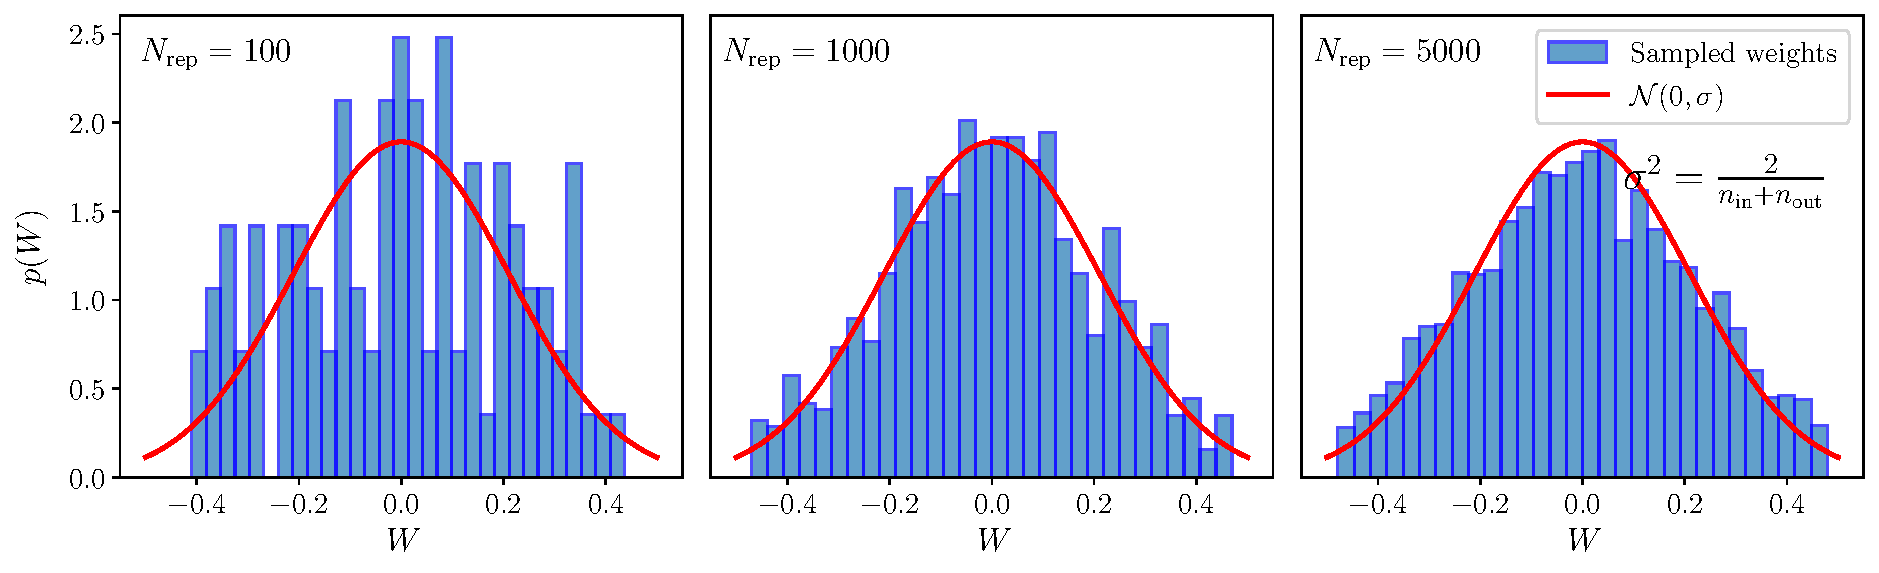
\includegraphics[width=0.95\textwidth]{section_2/weight_distribution.pdf}
  \caption{Sampled distribution of a selected weight in function of the
  number of replicas. The red line represent the underlying Gaussian distribution
  from which the weights are drawn. As the number of replicas is increased the 
  distribution of the weight converges to the expected Gaussian.}
  \label{fig:weight_distribution}
\end{figure}
% ===================================
The Glorot normal initialiser draws each weight and bias of the NN from independent Gaussian
distributions, denoted $p_w$ and $p_b$ respectively, centred at zero and with variances
rescaled by the number of nodes in adjacent layers,
\begin{equation}
    \label{eq:RescaledGlorotVariances}
    \frac{C^{(\ell)}_{w}}{\sqrt{n_{\ell-1} + n_{\ell}}}\, ,
    \quad \frac{C^{(\ell)}_{b}}{\sqrt{n_{\ell-1} + n_{\ell}}}\, .
\end{equation}
Following the NNPDF prescription, we have $C^{(\ell)}_{w}=C^{(\ell)}_{b}=1$.
Fig.~\ref{fig:weight_distribution} shows the binned distribution of a selected
weight in the network as a function of the number of replicas. Together with the
histogram, the underlying Gaussian, as dictated by the Glorot normal
initialisation, is also shown. The figure illustrates that the distribution of
the weights converges to the expected Gaussian as the number of replicas increases.

The probability distribution of the NN parameters induces a probability distribution for the
preactivations,
\begin{align}
    \label{eq:PreactAtInit}
    p\left(\phi^{(\ell)}\right)
      &= \int \mathcal{D}w\, p_w(w)\,
        \mathcal{D}b\, p_b(b)\, \prod_{i,\alpha}
        \delta\left(
          \phi^{(\ell)}_{i\alpha} - \sum_{j} w^{(\ell)}_{ij}
          \rho\left(\phi^{(\ell-1)}_{j\alpha}\right)
          - b^{(\ell)}_i
          \right)\, .
\end{align}
Note that, here and in what follows, $p(\phi^{(\ell)})$ denotes the joint probability for all the
$n_{\ell}\times\ngrid$ components of $\phi^{(\ell)}$,
\begin{align}
    \label{eq:ExplIndices}
    p\left(\phi^{(\ell)}\right) = p\left(\phi^{(\ell)}_{1,\alpha_1}, \phi^{(\ell)}_{2,\alpha_1}, \ldots,
        \phi^{(\ell)}_{n_\ell,\alpha_1}, \phi^{(\ell)}_{1,\alpha_2}, \ldots, \phi^{(\ell)}_{n_\ell,\alpha_2},
        \ldots,
        \phi^{(\ell)}_{n_\ell,\ngrid}\right)\, .
\end{align}
This duality between parameter-space and function-space provides a powerful framework to study
the behaviour of an ensemble of NNs, and in particular the symmetry properties of the distribution
$p(\phi^{(\ell)})$, see \eg~\cite{Maiti:2021fpy}. Working in parameter space, \ie\ computing the
expectation values of correlators of fields as integrals over the NN parameter, one can readily
show that
\begin{align}
    \label{eq:NeurRotInv}
    \mathbb{E}\left[
        R_{i_1j_1} \phi^{(n_\ell)}_{j_1 \alpha_1} \ldots
        R_{i_nj_n} \phi^{(n_\ell)}_{j_n \alpha_n}
    \right] =
    \mathbb{E}\left[
        \phi^{(n_\ell)}_{i_1 \alpha_1} \ldots
        \phi^{(n_\ell)}_{i_n \alpha_n}
    \right]\, ,
\end{align}
where $R$ is an orthogonal matrix in $\text{SO}(n_{\ell})$. Eq.\eqref{eq:NeurRotInv} implies
that the probability distribution in Eq.~\eqref{eq:PreactAtInit} is also invariant under rotations,
and therefore it can only be a function of $\text{SO}(n_{\ell})$ invariants. Therefore
\begin{align}
    \label{eq:PriorAction}
    p\left(\phi^{(n_\ell)}\right) =
        \frac{1}{Z^{(\ell)}} \exp\left(-S\left[\phi^{(\ell)}_{\alpha_1}
            \cdot \phi^{(\ell)}_{\alpha_2}\right]\right)\, ,
\end{align}
where
\begin{align}
    \label{eq:PhiInvariant}
    \phi^{(\ell)}_{\alpha_1}
            \cdot \phi^{(\ell)}_{\alpha_2} =
    \sum_{i=1}^{n_\ell} \phi^{(\ell)}_{i \alpha_1} \phi^{(\ell)}_{i \alpha_2}\, .
\end{align}
The action can be expanded in powers of the invariant bilinear,
\begin{align}
    \label{eq:ExpandAction}
    S\left[\phi^{(\ell)}_{\alpha_1}
            \cdot \phi^{(\ell)}_{\alpha_2}\right] =
        \frac12 \gamma^{(\ell)}_{\alpha_1\alpha_2}
            \phi^{(\ell)}_{\alpha_1} \cdot \phi^{(\ell)}_{\alpha_2} +
            \frac{1}{8 n_{\ell-1}} \gamma^{(\ell)}_{\alpha_1\alpha_2,\alpha_3\alpha_4}
            \phi^{(\ell)}_{\alpha_1} \cdot \phi^{(\ell)}_{\alpha_2} \,
            \phi^{(\ell)}_{\alpha_3} \cdot \phi^{(\ell)}_{\alpha_4} + O(1/n_{\ell-1}^2)\, ,
\end{align}
so that the probability distribution is fully determined by the couplings 
$\gamma^{(\ell)}$.\footnote{
    We have denoted {\em all}\ couplings by $\gamma^{{(\ell)}}$. Different couplings 
    are indentified by the number of indices, so that $\gamma^{(\ell)}_{\alpha_1\alpha_2}$ 
    is a two-point coupling, $\gamma^{(\ell)}_{\alpha_1\alpha_2,\alpha_3\alpha_4}$ is a four-point 
    coupling, etc. 
} 
In
Eq.~\eqref{eq:ExpandAction}, we have factored out inverse powers of $n_\ell$ for each coupling.
With this convention, and with the scaling of the parameters variances in
Eq.~\eqref{eq:RescaledGlorotVariances}, the couplings in the action are all $O(1)$
in the limit where $n_\ell\to\infty$.
As a consequence, the probability distribution at initialisation is a multidimensional Gaussian at
leading order -- \ie\ $\mathcal{O}(1)$ -- in $1/n_\ell$, with quartic corrections that are $O(1/n_\ell)$, while higher powers
of the invariant bilinear are suppressed by higher powers of the width of the layer. This power counting
defines an effective field theory, where deviations from Gaussianity can be computed in perturbation
theory to any given order in $1/n_\ell$, see \eg\ Ref.~\cite{Roberts:2021fes} for a detailed
presentation of these ideas. While the actual calculations become rapidly cumbersome, the
conceptual framework is straightforward.

At leading order, the second and fourth cumulant are respectively
\begin{align}
    &\langle \phi^{(\ell)}_{i_1,\alpha_1} \phi^{(\ell)}_{i_2,\alpha_2}\rangle
      = \delta_{i_1 i_2} K^{(\ell)}_{\alpha_1\alpha_2} + O(1/n_{\ell-1})\, , \\
    &\langle \phi^{(\ell)}_{i_1,\alpha_1} \phi^{(\ell)}_{i_2,\alpha_2}
      \phi^{(\ell)}_{i_3,\alpha_3} \phi^{(\ell)}_{i_4,\alpha_4}\rangle_c
      = O(1/n_{\ell-1})\, ,
\end{align}
where
\begin{equation}
    \label{eq:DefineKmat}
    K^{(\ell)}_{\alpha_1\alpha_2} = \left(\gamma^{(\ell)}\right)^{-1}_{\alpha_1\alpha_2}\, .
\end{equation}
The ``evolution'' of the couplings as we go deep in the NN, \ie\ the dependence of the couplings on
$\ell$, is governed by Renormalization Group (RG) equations, which preserve the power counting in
powers of $1/n_{\ell}$. At leading order,
\begin{align}
    K^{(\ell+1)}_{\alpha_1\alpha_2} &=
      \left.
      C_b^{(\ell+1)} + C_w^{(\ell+1)} \frac{1}{n_\ell}
      \langle \vec{\rho}^{\,(\ell)}_{\alpha_1} \cdot
      \vec{\rho}^{\,(\ell)}_{\alpha_2} \rangle
      \right|_{O(1)} \\
      \label{eq:RecursionForK}
      &= C_b^{(\ell+1)} + C_w^{(\ell+1)} \frac{1}{n_\ell}
      \langle \vec{\rho}^{\,(\ell)}_{\alpha_1} \cdot
      \vec{\rho}^{\,(\ell)}_{\alpha_2} \rangle_{K^{(\ell)}}\, ,
\end{align}
where
\begin{align*}
    \frac{1}{n_\ell}
      \langle \vec{\rho}^{\,(\ell)}_{\alpha_1} \cdot
      \vec{\rho}^{\,(\ell)}_{\alpha_2} \rangle_{K^{(\ell)}} =
    \int \prod_{\alpha}d\phi_\alpha\,
      \frac{e^{-\frac12 \left(K^{(\ell)}\right)^{-1}_{\beta_1\beta_2}
        \phi_{\beta_1} \phi_{\beta_2}}}
        {\left|2\pi K^{(\ell)}\right|^{1/2}}\,
        \rho(\phi_{\alpha_1}) \rho(\phi_{\alpha_2})\, .
\end{align*}
Eq.~\eqref{eq:RecursionForK} can be iterated using the NNPDF architecture,
yielding the covariance at initialisation for various depths. These are compared
with the empirical covariance computed from an ensemble of 100 replicas in
Fig.~\ref{Fig:KRecursionOne} for the first deep-layer and in
Fig.~\ref{Fig:KRecursionTwo} for the second-deep layer and output layer. The
agreement between the theoretical prediction and the empirical computation is
excellent, confirming the validity of the large-network expansion even for
networks of moderate size, as those used in the NNPDF fits.

\begin{figure}[t]
    \centering
    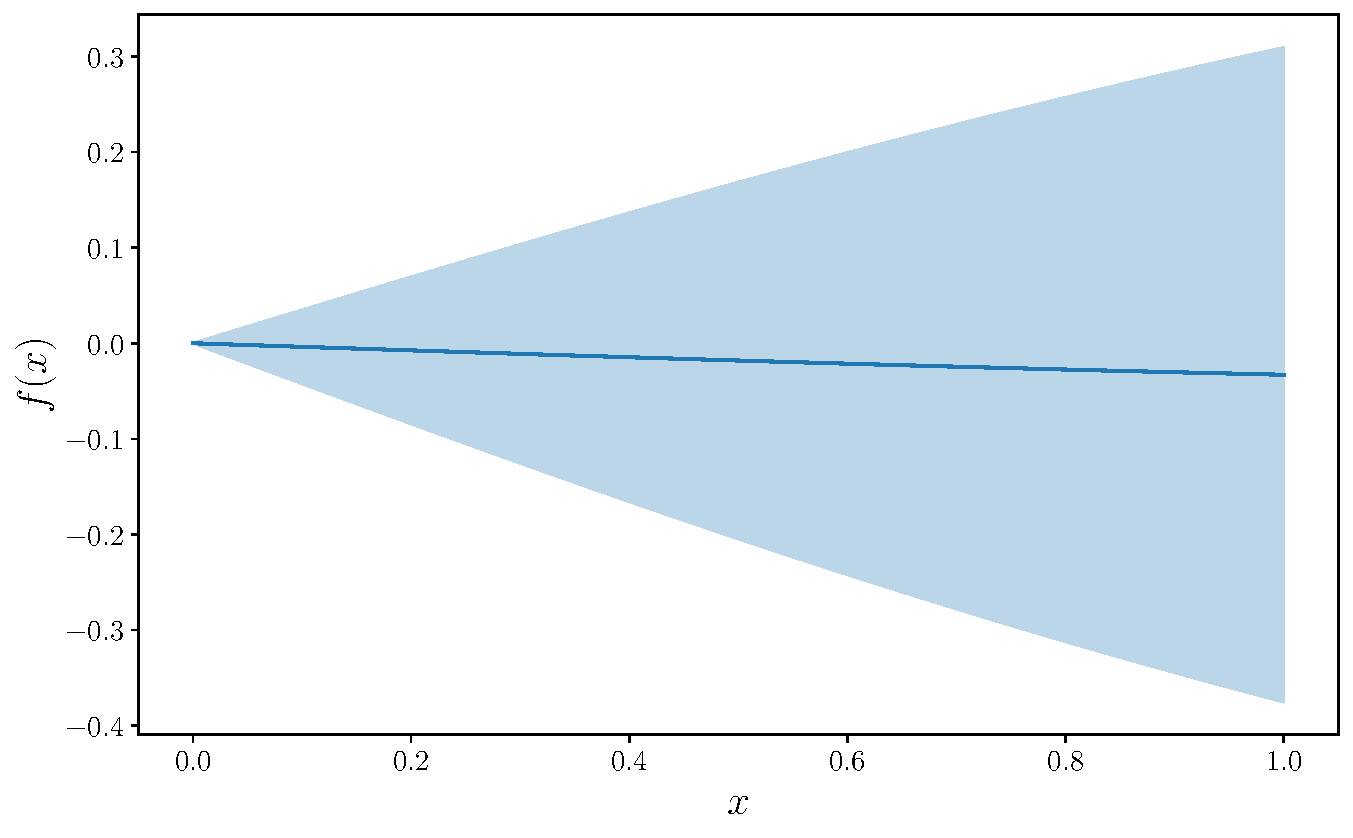
\includegraphics[width=0.45\textwidth]{section_2/prior.pdf}
    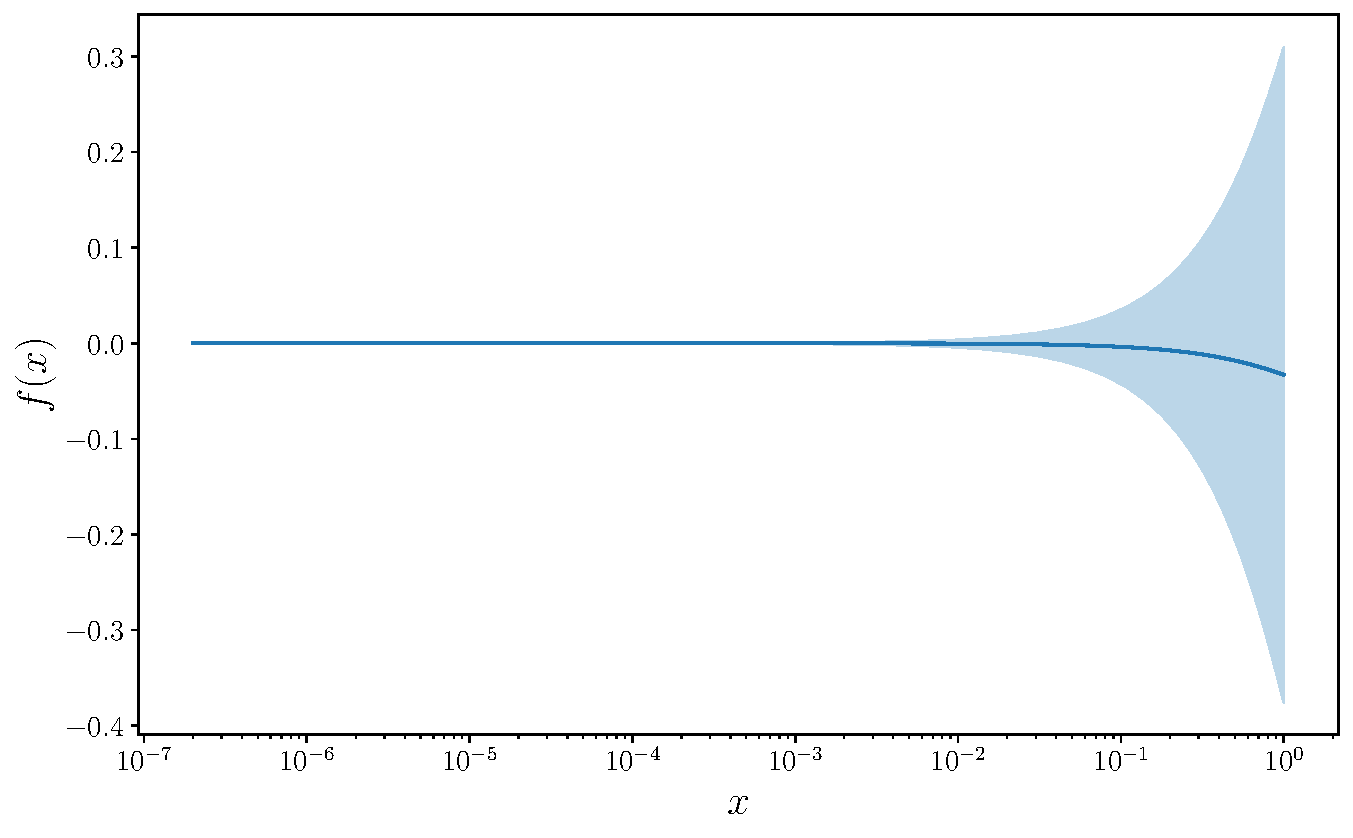
\includegraphics[width=0.45\textwidth]{section_2/prior_log.pdf}
    \caption{Ensemble of neural networks at initialisation in linear (left) and logarithm (right) scale.
    The blue line represents the mean value computed over an ensemble of 100 replicas, while the
    shaded band represents the one-sigma uncertainty computed as the variance over the same ensemble.
    In the figure, we show $xT_3$ as used in the following sections.}        
    \label{fig:prior} 
\end{figure}
\begin{figure}[t]
    \centering
    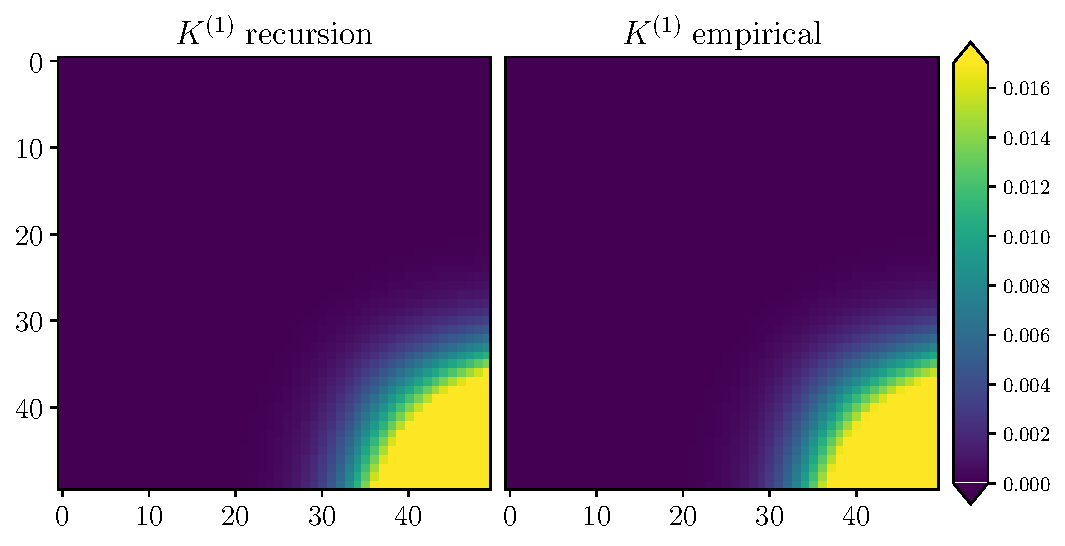
\includegraphics[scale=0.8]{section_2/K1_correlations.pdf}
    \caption{The empirical (left) and analytical (right) covariance matrices $K^{(1)}$ of the first layer
    of the NNPDF architecture. The covariance in the left panel is computed ``bootstrapping'' over an
    ensemble of 100 replicas, initialised using the Glorot normal distribution. The covariance in the right
    panel is obtained by solving Eq.~\eqref{eq:RecursionForK} numerically.
    \ldd{What is the level of the agreement?}
    \label{Fig:KRecursionOne}
    }
\end{figure}

\begin{figure}[t]
    \centering
    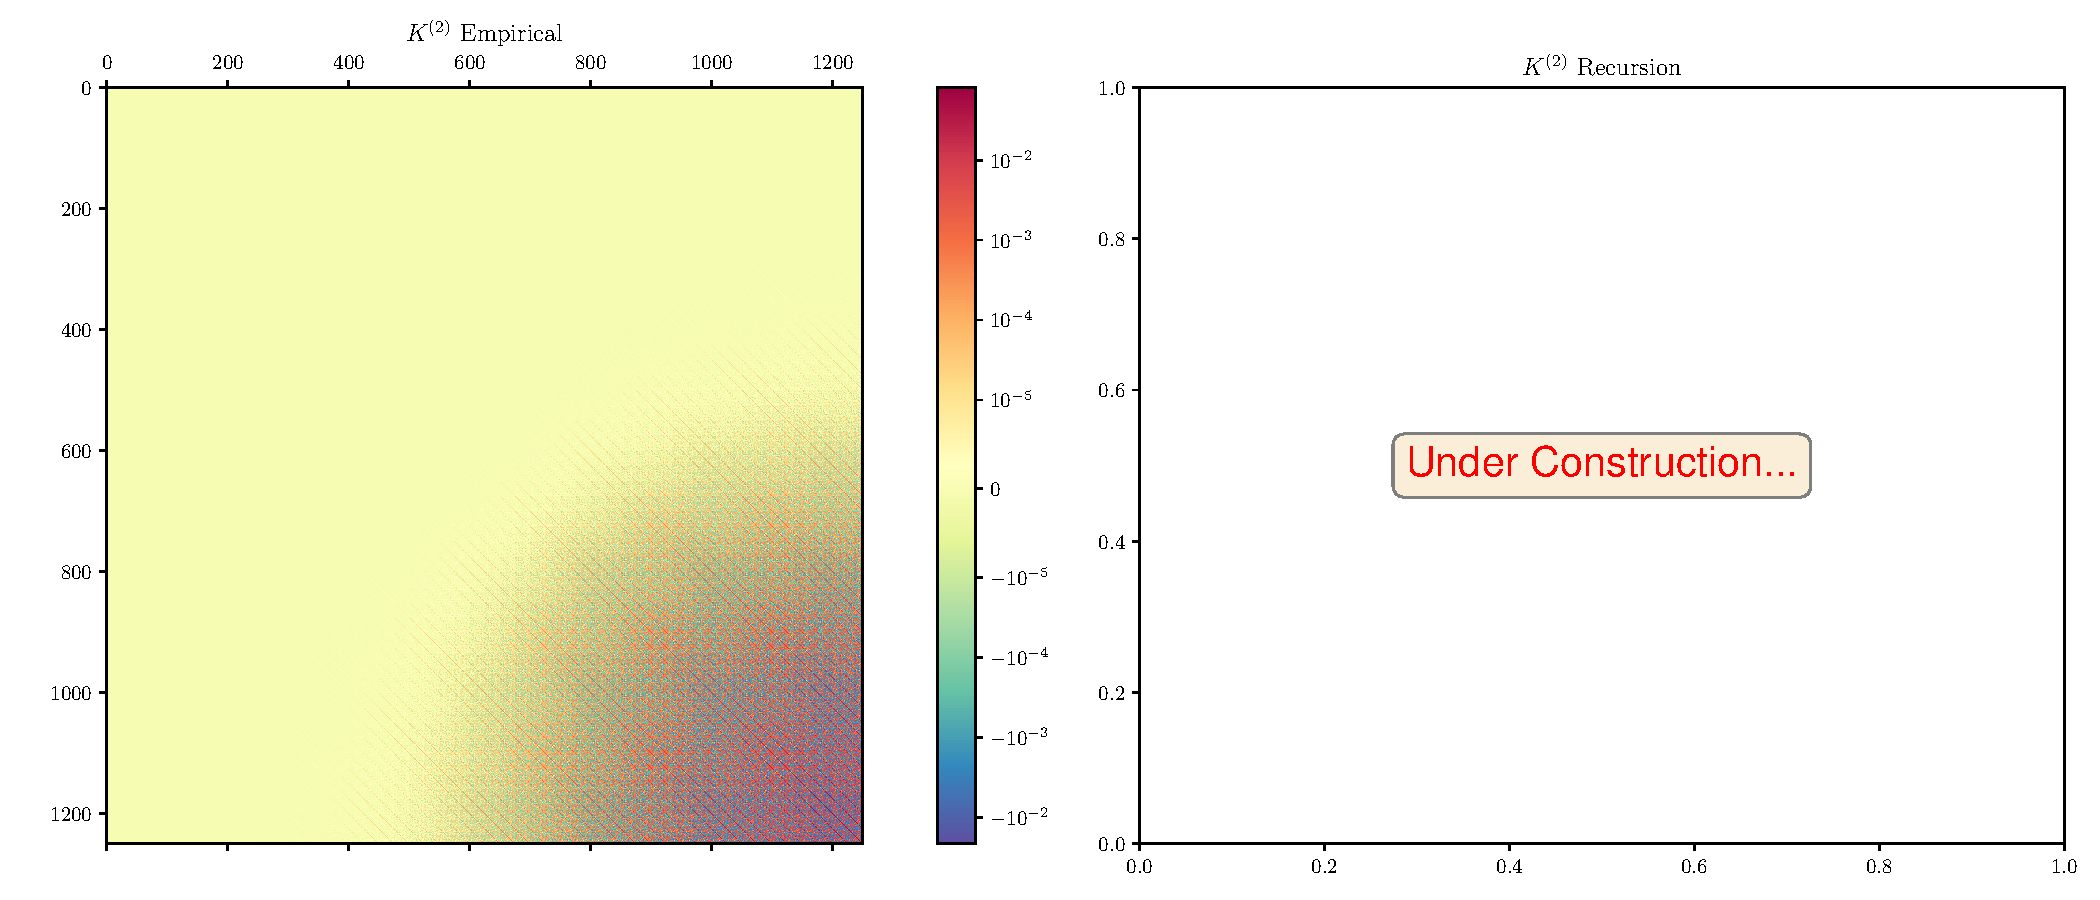
\includegraphics[scale=0.45]{section_2/K2_correlations.pdf}
    \hspace{0.5cm}
    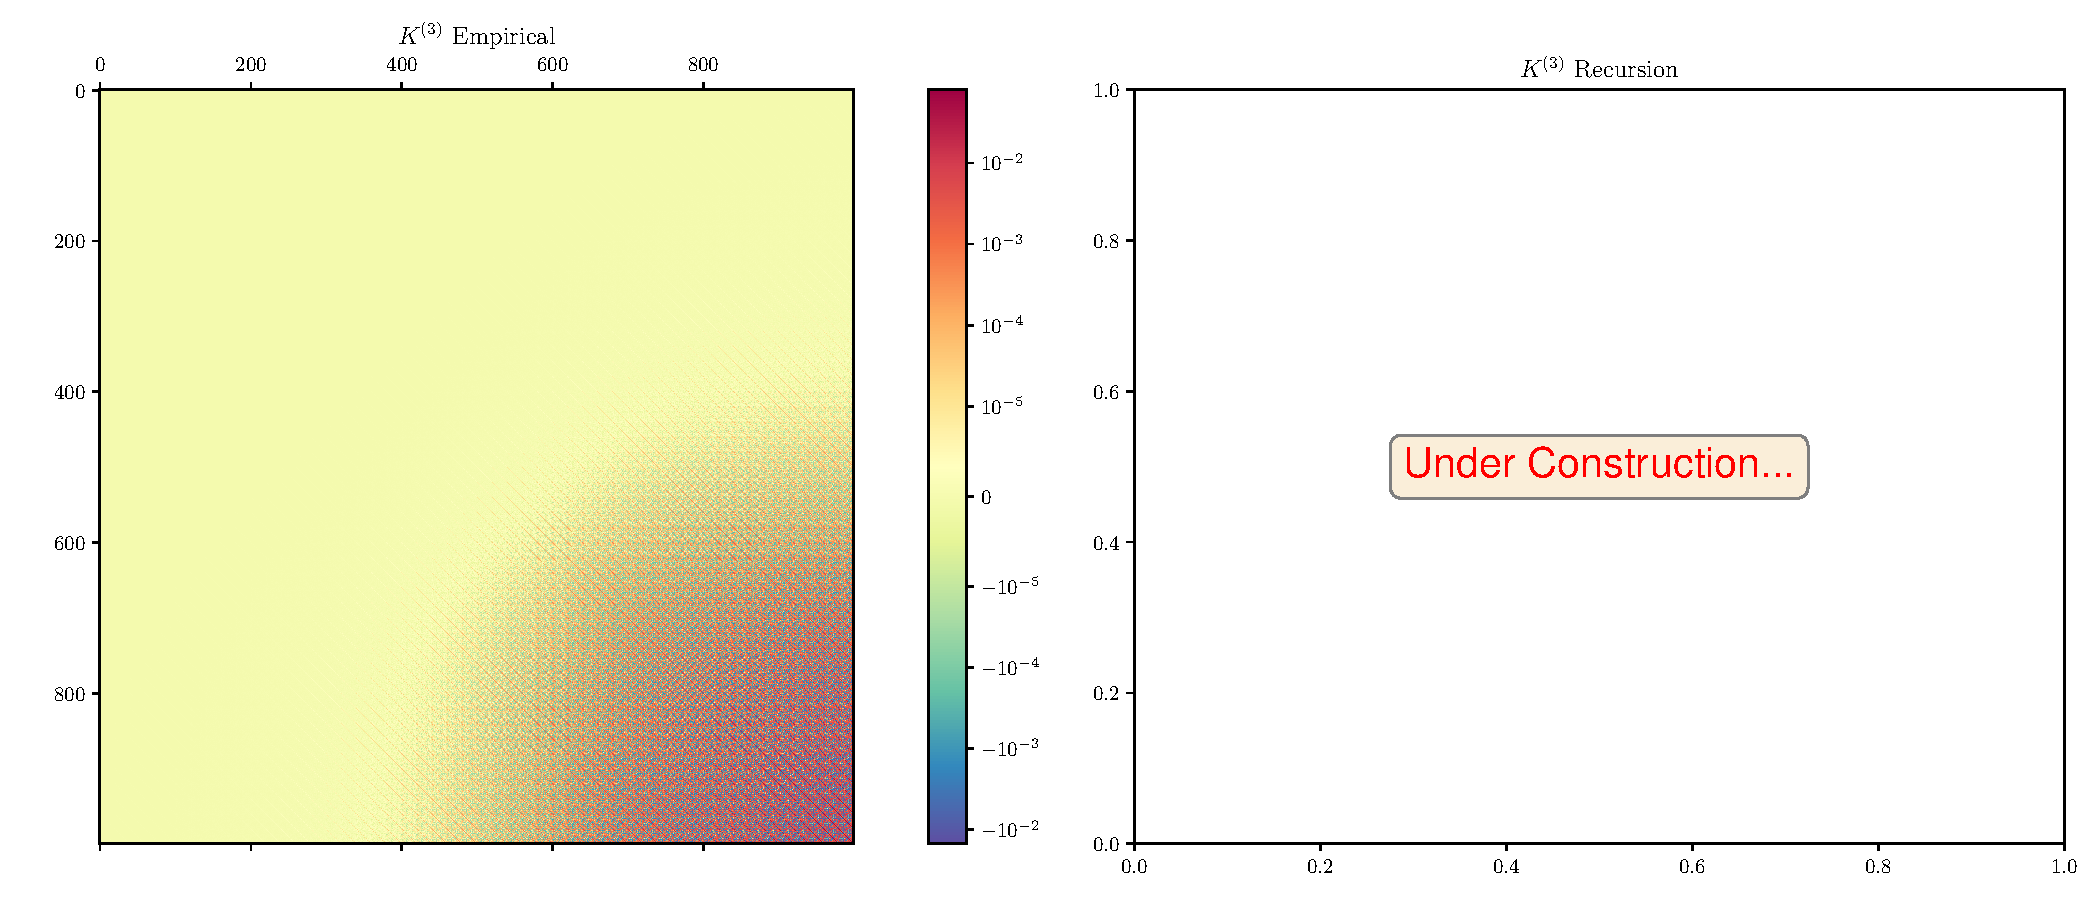
\includegraphics[scale=0.45]{section_2/K3_correlations.pdf}
    \caption{Same as Fig.~\ref{Fig:KRecursionOne}, but for the second (top) and
    third (bottom) layers of the NNPDF architecture.}
    \ldd{What is the level of the agreement?}
    \label{Fig:KRecursionTwo}
\end{figure}
\begin{figure}[t]
    \centering
    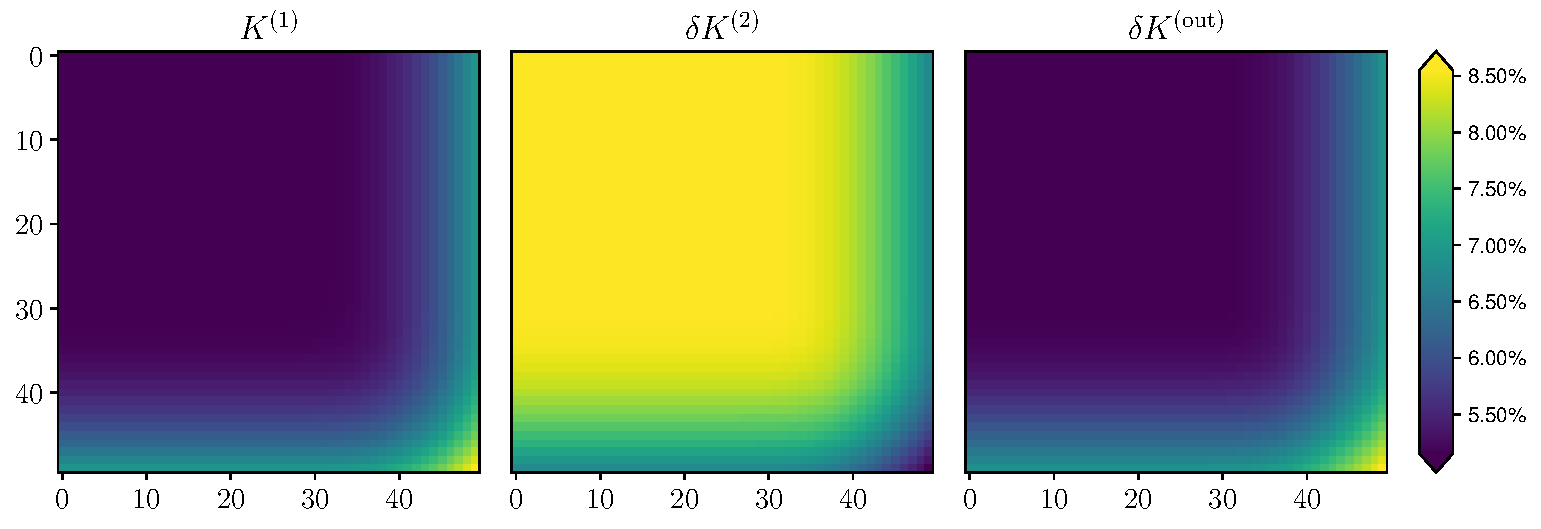
\includegraphics[width=0.9\textwidth]{section_2/delta_K.pdf}
    \caption{Here we show the relative difference between the empirical
    kernel computed from an ensemble of 100 replicas at initialisation
    and the theoretical prediction obtained by iterating
    Eq.~\eqref{eq:RecursionForK} for the three layers of the NNPDF architecture.
    \ac{Does this give more information than the previous plots?}}
\end{figure}


As a consequence of the symmetry of the probability distribution, the mean value
of the fields at initialisation needs to vanish, while their variance at each
point $x_\alpha$ is given by the diagonal matrix elements of $K^{(\ell)}$. In
the following, we will consider neural networks with the NNPDF architecture, but
will consider only one output layer. The mean and variance of the output at
initialisation are shown in Fig.~\ref{fig:prior} for an ensemble of
$\nreps=100$. The central value is computed as discussed above in
Eq.~\eqref{eq:ReplicaEnsemble},
\begin{align}
    \label{eq:MeanValAtInit}
    \bar{f}_{i\alpha} = \bar{f}_{i}(x_\alpha) = \frac{1}{\nreps} \sum_{k=1}^{\nreps} f^{(k)}_i(x_\alpha)\, ,
\end{align}
and the variance $\sigma^2_{i\alpha}$ is computed using the same formula with
\begin{align}
    \label{eq:VarAtInit}
    O(f) = \frac{\nreps}{\nreps-1} \left(f_i(x_\alpha) - \bar{f}_{i}(x_\alpha)\right)^2\, .
\end{align}

\FloatBarrier
